\documentclass[tikz]{standalone}

\usepackage{transparent}
\usepackage{nicematrix}
\usetikzlibrary{matrix, fit}
\usetikzlibrary{backgrounds}
\usetikzlibrary{positioning}
\usetikzlibrary{decorations.pathreplacing}

\newlength{\mycellheight}
\newlength{\innermargin}
\newlength{\cornerrad}
\newlength{\vsep}
\newlength{\msep}  % Offset from center
\newlength{\hsep}  % Offset between blocks
\newlength{\thirdlevelsep}

\newcommand{\0}{{\transparent{0} \resizebox{\mycellheight}{\mycellheight}{0}}}

\begin{document}
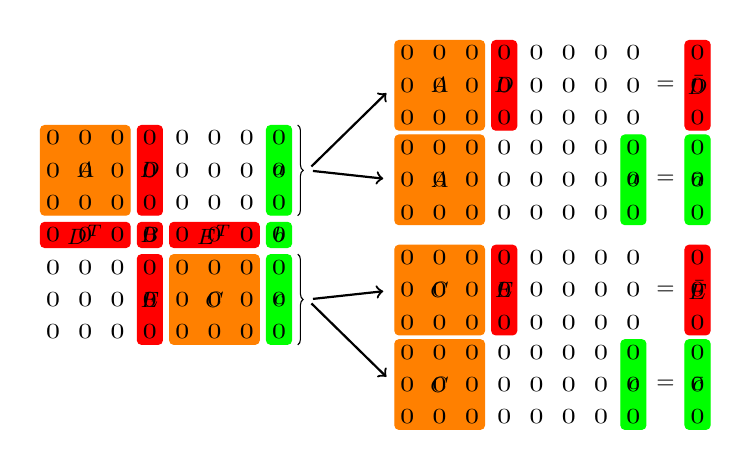
\begin{tikzpicture}
    
    \setlength{\mycellheight}{0.5em}
    \setlength{\innermargin}{-0.15em}
    \setlength{\cornerrad}{1.5pt}
    \setlength{\vsep}{1.2cm}
    \setlength{\msep}{0.7cm}
    \setlength{\hsep}{4.5cm}
    % \setlength{\thirdlevelsep}{\vsep/2}

    \matrix[matrix of math nodes, draw=none] (m0) 
    {
        \0&\0&\0&\0&\0&\0&\0&\0\\
        \0&\0&\0&\0&\0&\0&\0&\0\\
        \0&\0&\0&\0&\0&\0&\0&\0\\
        \0&\0&\0&\0&\0&\0&\0&\0\\
        \0&\0&\0&\0&\0&\0&\0&\0\\
        \0&\0&\0&\0&\0&\0&\0&\0\\
        \0&\0&\0&\0&\0&\0&\0&\0\\
    };
    \matrix[matrix of math nodes, draw=none] at (\hsep,\msep+\vsep) (m1) 
    {
        \0&\0&\0&\0&\0&\0&\0&\0\\
        \0&\0&\0&\0&\0&\0&\0&\0\\
        \0&\0&\0&\0&\0&\0&\0&\0\\
    };
    \matrix[matrix of math nodes, draw=none] at (\hsep,\msep) (m2) 
    {
        \0&\0&\0&\0&\0&\0&\0&\0\\
        \0&\0&\0&\0&\0&\0&\0&\0\\
        \0&\0&\0&\0&\0&\0&\0&\0\\
    };
    \matrix[matrix of math nodes, draw=none] at (\hsep,-\msep) (m3) 
    {
        \0&\0&\0&\0&\0&\0&\0&\0\\
        \0&\0&\0&\0&\0&\0&\0&\0\\
        \0&\0&\0&\0&\0&\0&\0&\0\\
    };
    \matrix[matrix of math nodes, draw=none] at (\hsep,-\msep -\vsep) (m4) 
    {
        \0&\0&\0&\0&\0&\0&\0&\0\\
        \0&\0&\0&\0&\0&\0&\0&\0\\
        \0&\0&\0&\0&\0&\0&\0&\0\\
    };
    \matrix[matrix of math nodes, draw=none] at (1.5\hsep,\msep +\vsep) (m5) 
    { \0\\ \0\\ \0\\ };
    \matrix[matrix of math nodes, draw=none] at (1.5\hsep,\msep) (m6) 
    { \0\\ \0\\ \0\\ };
    \matrix[matrix of math nodes, draw=none] at (1.5\hsep,-\msep) (m7) 
    { \0\\ \0\\ \0\\ };
    \matrix[matrix of math nodes, draw=none] at (1.5\hsep,-\msep -\vsep) (m8) 
    { \0\\ \0\\ \0\\ };

    \begin{scope}[on background layer]
        \foreach \x in {0,1,3} {
            \node[fit=(m\x-1-4)(m\x-3-4), draw=red, fill=red, rounded corners=\cornerrad, inner sep=\innermargin] (D\x) {};
        }
        % Red blocks
        \node at (D0) {\footnotesize $D$};
        \node at (D1) {\footnotesize $D$};
        \node at (D3) {\footnotesize $E$};
        \node[fit=(m0-5-4)(m0-7-4), draw=red, fill=red, rounded corners=\cornerrad, inner sep=\innermargin] (E) {};
        \node[fit=(m0-4-1)(m0-4-3), draw=red, fill=red, rounded corners=\cornerrad, inner sep=\innermargin] (Dt) {};
        \node[fit=(m0-4-5)(m0-4-7), draw=red, fill=red, rounded corners=\cornerrad, inner sep=\innermargin] (Et) {};
        \node[fit=(m0-4-4)(m0-4-4), draw=red, fill=red, rounded corners=\cornerrad, inner sep=\innermargin] (B) {};

        \foreach \m in {5,7} {
            \node[fit=(m\m-1-1)(m\m-3-1), draw=red, fill=red, rounded corners=\cornerrad, inner sep=\innermargin] (Dbar\m) {};
        }

        % Orange blocks
        \foreach \x in {0,1,2,3,4} {
            \node[fit=(m\x-1-1)(m\x-3-3), draw=orange, fill=orange, rounded corners=\cornerrad, inner sep=\innermargin] (A\x) {};
        }
        \foreach \x in {0,1,2} {
            \node at (A\x) {\footnotesize $A$};
        }
        \node[fit=(m0-5-5)(m0-7-7), draw=orange, fill=orange, rounded corners=\cornerrad, inner sep=\innermargin] (C) {};
        \node at (A3) {\footnotesize $C$};
        \node at (A4) {\footnotesize $C$};

        % Green blocks
        \foreach \x in {0,2,4} {
            \node[fit=(m\x-1-8)(m\x-3-8), draw=green, fill=green, rounded corners=\cornerrad, inner sep=\innermargin] (a\x) {};
        }
        \foreach \x in {1,3} {
            \node[fit=(m\x-1-8)(m\x-3-8), rounded corners=\cornerrad, inner sep=\innermargin] (a\x) {};
        }
        \node at (a0) {\footnotesize $a$};
        \node at (a2) {\footnotesize $a$};
        \node at (a4) {\footnotesize $c$};
        \node[fit=(m0-4-8)(m0-4-8), draw=green, fill=green, rounded corners=\cornerrad, inner sep=\innermargin] (b0) {};
        \node[fit=(m0-5-8)(m0-7-8), draw=green, fill=green, rounded corners=\cornerrad, inner sep=\innermargin] (c0) {};
        \foreach \m in {6,8} {
            \node[fit=(m\m-1-1)(m\m-3-1), draw=green, fill=green, rounded corners=\cornerrad, inner sep=\innermargin] (abar\m) {};
        }

    \end{scope}
    \node at (B) {\footnotesize $B$};
    \node at (C) {\footnotesize $C$};
    \node at (Dt) {\footnotesize $D^T$};
    \node at (E) {\footnotesize $E$};
    \node at (Et) {\footnotesize $E^T$};
    \node at (b0) {\footnotesize $b$};
    \node at (c0) {\footnotesize $c$};
    \node at (Dbar5) {\footnotesize $\bar{D}$};
    \node at (Dbar7) {\footnotesize $\bar{E}$};
    \node at (abar6) {\footnotesize $\bar{a}$};
    \node at (abar8) {\footnotesize $\bar{c}$};

    \foreach \x in {a,c} {
        \draw[decorate,decoration={brace,amplitude=2pt, raise=2pt, aspect=0.5}] 
            (\x0.north east) -- (\x0.south east) 
            node[pos=0.5,right,anchor=center,xshift=2pt] (\x brace) {};
    }
    \draw[->,thick, shorten <=0.2em, shorten >=0.4em] (abrace.east)--(A1.west);
    \draw[->,thick, shorten <=0.2em, shorten >=0.4em] (abrace.east)--(A2.west);
    \draw[->,thick, shorten <=0.2em, shorten >=0.4em] (cbrace.east)--(A3.west);
    \draw[->,thick, shorten <=0.2em, shorten >=0.4em] (cbrace.east)--(A4.west);

    \node[left] at (Dbar5.west) {\footnotesize $=$};
    \node[left] at (Dbar7.west) {\footnotesize $=$};
    \node[left] at (abar6.west) {\footnotesize $=$};
    \node[left] at (abar8.west) {\footnotesize $=$};
    % \node[right] at (a1.east) {\footnotesize $\implies \bar{D}$};
    % \node[right] at (a2.east) {\footnotesize $\implies \bar{a}$};
    % \node[right] at (a3.east) {\footnotesize $\implies \bar{E}$};
    % \node[right] at (a4.east) {\footnotesize $\implies \bar{c}$};

    % \draw[decorate,decoration={brace,amplitude=2pt, raise=2pt, aspect=0.4}] 
    %     (c0.north east) -- (c0.south east) 
    %     node[pos=0.4,right,anchor=west,xshift=4pt, inner sep=0.1em] (l2) {};


\end{tikzpicture}
\end{document}